\documentclass{tufte-book}

\usepackage{amsmath, amsthm}
\usepackage{graphicx}
\setkeys{Gin}{width=\linewidth,totalheight=\textheight,keepaspectratio}
\graphicspath{{graphics/}}

\title{STATS 244 \\ Homework 4}
\author{Joe Seidel}
\date{\today}

\usepackage{booktabs}
\usepackage{units}
\usepackage{fancyvrb}
\fvset{fontsize=\normalsize}
\usepackage{multicol}
\usepackage{lipsum}
\usepackage{pdfpages}
\usepackage{tikz}
\usepackage{wasysym}

\newcommand{\doccmd}[1]{\texttt{\textbackslash#1}}% command name -- adds backslash automatically
\newcommand{\docopt}[1]{\ensuremath{\langle}\textrm{\textit{#1}}\ensuremath{\rangle}}% optional command argument
\newcommand{\docarg}[1]{\textrm{\textit{#1}}}% (required) command argument
\newenvironment{docspec}{\begin{quote}\noindent}{\end{quote}}% command specification environment
\newcommand{\docenv}[1]{\textsf{#1}}% environment name
\newcommand{\docpkg}[1]{\texttt{#1}}% package name
\newcommand{\doccls}[1]{\texttt{#1}}% document class name
\newcommand{\docclsopt}[1]{\texttt{#1}}% document class option name
\DeclareMathOperator{\proj}{proj}
\newcommand{\vct}{\mathbf}


\newcommand{\dprod}[2]{\langle #1, #2 \rangle}
\newcommand{\Var}{\mathrm{Var}}
\newcommand{\Cov}{\mathrm{Cov}}
\newcommand{\MSE}{\mathrm{MSE}}
\newcommand{\MLE}{\mathrm{MLE}}

\newtheoremstyle{mytheoremstyle} % name
	{\topsep}		% Space above
	{\topsep}		% Space below
	{\itshape}		% Body font
	{}			% Indent amount
	{\bfseries}	% Theorem head font
	{\textnormal{:}}	% Punctuation after theorem head
	{.5em}		% Space after theorem head
	{}			%Theorem headspec
\theoremstyle{mytheoremstyle}
\newtheorem*{thm}{Thm.}

\newtheoremstyle{mylemstyle} % name
	{\topsep}		% Space above
	{\topsep}		% Space below
	{\itshape}		% Body font
	{}			% Indent amount
	{\bfseries}	% Theorem head font
	{\textnormal{:}}	% Punctuation after theorem head
	{.5em}		% Space after theorem head
	{}			%Theorem headspec
\theoremstyle{mylemstyle}
\newtheorem*{lem}{Lem.}


\newtheoremstyle{mydefstyle} % name
	{\topsep}		% Space above
	{\topsep}		% Space below
	{\normalfont}	% Body font
	{}			% Indent amount
	{\bfseries}	% Theorem head font
	{\textnormal{:}}	% Punctuation after theorem head
	{.5em}		% Space after theorem head
	{}			%Theorem headspec
\theoremstyle{mydefstyle}
\newtheorem*{mydef}{Def.}
\newtheorem*{ex}{E.g.}

\begin{document}

\maketitle
\pagenumbering{gobble}
\newpage
\pagenumbering{arabic}

\subsection{Question 1}
Let $Z \sim N(0,1)$, a stand normal distribution and let $X \sim N(\mu \sigma^2)$.  Let $\Phi(z)$ be the cdf of $Z$.  Suppose $X \sim N(-4, 16)$; find.

It helps to know that
\[ P(X < x) = \Phi\Big(\frac{x-\mu}{\sigma}\Big). \]

\begin{enumerate}
\item $P(X > 2)$.
\begin{align*}
P(X > 2) &= 1 - P(X < 2)
&= 1 - \Phi\Big(\frac{2- (-4)}{\sqrt{16}}\Big)\\
&= 1 - .9332\\
&= .0688\\
\end{align*}

\item $P(0 < X < 4)$
\begin{align*}
    P(0 < X < 4) &= P(X<4) - P(X<0)\\
    &= \Phi\Big(\frac{4 -(-4)}{4}\Big) - \Phi\Big(\frac{0 -(-4)}{4}\Big) \\
    &= .1539
\end{align*}

\item $P(|X+3| \geq 3)$
\begin{align*}
    P(|X+3| \geq 3) &= P(X \geq 0) + P(X \leq -6)\\
    &= 1-\Phi\Big(\frac{4}{4}\Big) + \Phi\Big(\frac{-2}{4}\Big)\\
    &= .1587 + .3085\\
    &= .4672
\end{align*}

\item $P(X \leq 0 \text{ or } X \geq 3)$
\begin{align*}
    P(X \leq 0 \text{ or } X \geq 3) &= P(X \leq 0) + P(X \geq 3)\\
    &= \Phi\Big(\frac{4}{4}\Big) + 1 - \Phi\Big(\frac{7}{4}\Big)\\
    &= .8413 + .0003\\
    &= .8416\\
\end{align*}

\end{enumerate}


\subsection{Question 2}
Based on student A's performace during the first two weeks of a course, the professor has approximately a normal $N(70, 8^2)$ prior distribution about the student's true ability, on a scale of 0 to 100.  Consider the midterm examination as an error-prone measure of the student's true ability, where if the true ability is $x$, the examination score can be modeled as approximately normally distributed, $N(x,6^2)$.  The student scores 90 on the midterm.

\begin{enumerate}
\item What are the posterior expectaion and the probability that the student's true ability is above 85?

\newthought{We have} the following information.
    \[f(\theta) \sim N(70, 8^2) \]
 and
    \[f(x\mid \theta)\sim N(x, 6^2)\]

Using Bayes, $f(\theta\mid X) \propto f(x\mid \theta)f(\theta)$ the posterior distribution is

\[ (\theta\mid X) = \frac{1}{\sqrt{2\pi}B}e^{\frac{(\theta-A)^2}{2B^2}} \]
Where
\[ A = \frac{6^2(70) + 8^2(90)}{6^2 + 8^2} \]
and
\[B^2 = \frac{6^2*8^2}{6^2 + 8^2} \]

Which give us a $N(82.8, 23.4)$ posterier distribution and means posterior of expectation of the student's true ability it $82.8$.  Using the the method from question 1, there is a .4625 probability that the students true ability is above $85$.

\item Above 90?

.3792

\end{enumerate}


\subsection{Question 3}
A "psychic" uses a five-card deck of cards to demenonstrate ESP, and claims to be able to guess a card correctly with probability .5.  A single experiment consists of making five guesses, reshuffling the deck after each guess.  The experiment is treid and the "pyschic" guesses correctly 3 times out of give.  Assuming the only two possibilities are "ESP" and "ordinary guessing", how how must the a priori ability be that "psychic" has ESP is at alteast .7?

\newthought{Let} $P(\theta)$ be the prior probability that an individual has ESP that we wish to find.

Bayes thereom is
\[P(\theta \mid X) = \frac{P(X \mid \theta) P(\theta)}{\sum_{i=1}^2 P(X\mid \theta_i) P(\theta_i)}. \]

Where we can think of $P(\theta_1)= P(\theta)$ and $P(\theta_2) = 1-P(\theta)$

Plugging in the observed data along with guessing probabilities provided.

\[ P(X=3 \mid \theta) = \binom{5}{3}(.5)^3(.5)^2 = .3125 \]
and
\[ P(X=3 \mid \theta_2) = \binom{5}{3}(.2)^3(.8)^2 = .0512. \]

We can plug these values into Bayes and solve for $P(\theta \mid X) \leq .7$.  Ie

\[.7 \leq \frac{.3125P(\theta)}{.3125 P(\theta) + .0512(1-P(\theta))}\]

Which gives $P(\theta) \geq .276$



\subsection{Question 4}

Suppose $\hat{\theta}_1$ and $\hat{\theta}_2$ are uncorrelated and both are unbiased estimators of $\theta$, and that $\Var(\hat{\theta}_1) = 2\Var(\hat{\theta}_2)$.

\begin{enumerate}

\item Show that for any constant $c$, the weighted average $\hat{\theta}_3 = c\hat{\theta}_1 + (1-c)\hat{\theta}_2$ is an unbiased estimator of $\theta$.

\begin{align*}
E(\hat{\theta}_3) &= cE(\hat{\theta}_1) + (1-c)E(\hat{\theta}_2)\\
&= c\theta + (1-c)\theta\\
&= \theta\\
\end{align*}

Hence $B(\hat{\theta}_3) = 0$.

\item Find $c$ for which $\hat{\theta}_3$ has the smallest MSE.

The MSE of $\hat{\theta}_3$ is

\[ c^2\Var(\hat{\theta}_1) + (1-c)^2\Var(\hat{\theta}_2) \]

We can find the value, $c$, that minimizes MSE by evaulating.

\begin{align*}
MSE(\hat{\theta}_3) &= c^2\Var(\hat{\theta}_1) + (1-c)^2\Var(\hat{\theta}_2)\\
&=c^2 2\Var(\hat{\theta}_2) + (1-c)^2\Var(\hat{\theta}_2)\\
&=\Var(\hat{\theta}_2)(3c^2 - 2c + 1)\\
\end{align*}

Setting the above equal to $0$ results in $c=\frac{1}{3}$.  Furthermore, the second derivative of the MSE is positive so we can confirm that $c$ minimizes.

\item Are there any values of $c$, $0 \leq c \leq 1$ for which $\hat{\theta}_3$ is better (in the sense of MSE) than both $\hat{\theta}_1$ and $\hat{\theta}_2$

\newthought{We are} given that $\Var(\hat{\theta}_2)$ is less than $\Var(\hat{\theta}_1)$.  Since the bias as zero, the MSE is just the variance of each estimator.

Considering again the result from the question above...
\[
\text{MSE }\hat{\theta}_3 = \Var(\hat{\theta}_2)(3c^2 - 2c +1)
\]

implies that $0< c < \frac{2}{3}$ will do better in the sene of MSE than the other two estimators.

\end{enumerate}

\subsection{Question 5}
Consider observing $X$ from the density $f_\theta(x)=\frac{2}{\theta^2}(\theta-x)$, where $0<x<\theta$ and $\theta>0$ is unkown.

\begin{enumerate}
\item Verify that $f_\theta$ is indeed a valid density for all $\theta > 0$.

\begin{align*}
\int_0^\theta f_\theta(x)dx &= \int_0^\theta \frac{2}{\theta^2}(\theta-x)dx\\
&= \frac{2}{\theta^2}\int_0^\theta (\theta-x)dx\\
&= \frac{2}{\theta^2}[\theta^2 -  \frac{\theta^2}{2}]\\
&= 1\\
\end{align*}

\item Find the MLE of $\theta$ based on $X$.  Find the bias, the variance and the mean squared error of the MLE.

\newthought{The} MLE of $\theta$ can be found by solving $\frac{d}{d\theta}L(\theta) = 0$.

\begin{align*}
\frac{d}{d\theta}L(\theta) &= \frac{d}{d\theta}\frac{2}{\theta^2}(\theta-x)\\
&= 2 (\frac{d}{d\theta}\theta^{-1} - x\theta^{-2}\\
&= 4x\theta^{-3} - 2\theta^{-2}
\end{align*}

Setting the above to $0$ yields

\[
4x\theta^{-3} = 2\theta^{-2}.
\]

Hence $\hat{\theta} = 2X$.  Furthermore the second derivative of $L(\theta)$ is negative when $\theta=2x$ so we can be sure that this is a maximum when.

To find the bias, variance and MSE, tt helps to know the variance and expectation of $X$ which can be calculated from the given density.  Hence,
\begin{align*}
E(X) &= \frac{\theta}{3}\\
\Var(X) &= \frac{\theta^2}{18}\\
\end{align*}

\begin{align*}
B(\hat{\theta}) &= E(\hat{\theta}) - \theta\\
&= E(2X) - \theta\\
&= 2E(X) - \theta\\
&= 2(\frac{\theta}{3}) - \theta\\
&= -\frac{\theta}{3}
\end{align*}

\begin{align*}
\Var(\hat{\theta}) &= \Var(2X)\\
&= 2^2\Var(X)\\
&= \frac{4\theta^2}{9}\\
\end{align*}

\begin{align*}
\MSE(\hat{\theta}) &= \Var(\hat{\theta}) + B(\hat{\theta})^2\\
&=\frac{5\theta^2}{9}\\
\end{align*}

\item For the estimator $cX$ for $\theta$ (assume $c > 0$), find the bias, the variance and the mean squeated error of the estimator as a function of $\theta$.  For what value of $c$ is $cX$ unbiased?  For what value of $c$ is the mean squared error minimized?  Plot the mean square error as a function of c.
\begin{align*}
B(cX) &= E(cX) - \theta\\
&= cE(X) - \theta\\
&= c(\frac{\theta}{3}) - \theta\\
&= \frac{\theta(c - 3)}{3}\\
\end{align*}
\begin{align*}
\Var(cX) &= c^2\Var(X)\\
&= \frac{c^2\theta^2}{18}\\
\end{align*}
\begin{align*}
\MSE(cX) &= \Var(cX) + B(cX)^2\\
&= \frac{\theta^2(c^2 - 4c + 6)}{6}\\
\end{align*}

From the above, $cX$ is unbiased when $c=3$.  When $c=2$ the MSE is minized.

Plotting the MSE as a function of $c$ keeping fixing $\theta$ at a view values yields.

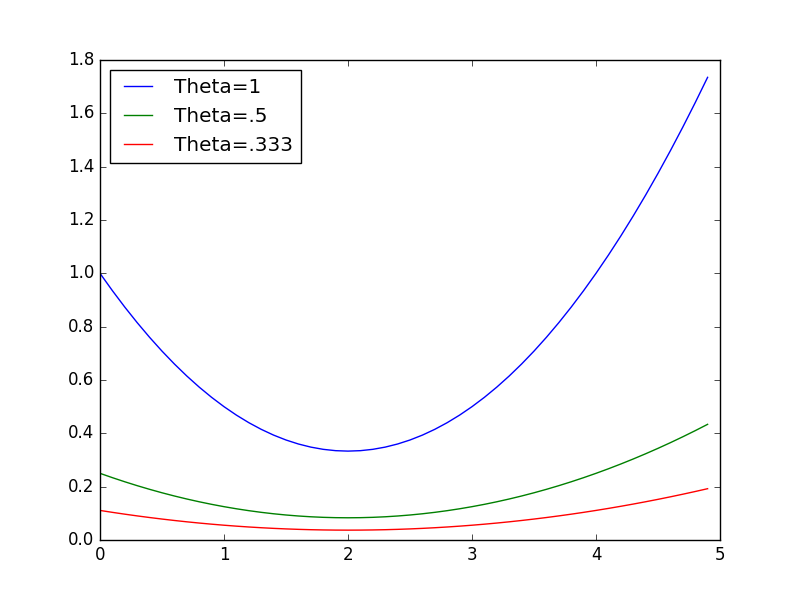
\includegraphics{q5}

\item Find the value of $c \neq \frac{1}{2}$ such that $cX$ has the same mean squared error as $\frac{1}{2}X$.  Call this value $c'$.  Discus which estimator of $\theta$ your prefer, $\frac{1}{2}X$ or $c'X$.

\newthought{Using} what we know about the $\MSE(cX)$ as a function of $c$,\\
 $c'=\frac{7}{2}$.

Compairing the two, $c'$ has a larger variance but smaller bias than $\frac{1}{2}X$.  So there is a tradeoff between the two, but I'd prefer the estimator with the smaller variance.

\end{enumerate}


\subsection{Question 6}
Suppose the data consist of a signle number $X$, and the model is that $X$ has the following probabilty density:

\[ f(x \mid \theta) = (1+x\theta)/2 \text{ for } -1 \leq x \leq 1;=0 \text{ otherwise.} \]

Supposing the possible values of $\theta$ are $0 \leq \theta \leq 1$; find the maximum likelihood estimate of $\theta$, $\hat{\theta}$, and its (exact) probability distibution.  Is the MLE unbiased?  Find its bias and MSE.

\newthought{Find} the MLE for sample variables of X.
For $X=0.5$
\[ \frac{d}{d\theta}L(\theta) = .25 \]

For $X=-0.5$
\[ \frac{d}{d\theta}L(\theta) = -.25 \]

Which suggests that $\MLE(\theta) = 0$.

The bias is $-\theta$.  The MSE is $\theta^2$


\subsection{Question 7}
Suppose we observe $X \sim \text{Unif}(0,\theta)$, $\theta > 0$.

\begin{enumerate}

\item Find the mle of $\theta$.

\[ p(x) = \frac{1}{\theta} \text{ for }{ \theta > 0} \]
\[ p(x \mid \theta) = \frac{1}{\theta} \text{ for } x=1,2,3...,\theta \]

\[ L(\theta) = \frac{1}{\theta} \text{ for }\theta \geq x \]

\item Find the mean squared error of the mle $\hat{\theta}$; that is $E_\theta\{(\hat{\theta} - \theta)^2\}$

First, find the bias and variance of $X$.
\begin{align*}
B(\hat{\theta}) &= E(X) - \theta\\
&= \frac{1+\theta}{2} - \theta\\
&= \frac{1-\theta}{2}
\end{align*}
\begin{align*}
\Var(X) &= E(X^2) - E(X)^2\\
&= \frac{(\theta+1)(2\theta+1)}{6} - \Big(\frac{\theta + 1}{2}\Big)^2\\
\end{align*}
\begin{align*}
\MSE(\hat{\theta}) &= \frac{(\theta+1)(2\theta+1)}{6} - \Big(\frac{\theta + 1}{2}\Big)^2 + \Big(\frac{1-\theta}{2}\Big)^2\\
&= \frac{2\theta^2 - 3\theta +1}{6}\\
\end{align*}

\item Find the constant $c$ that makes $cX$ an unbiased extimate of $\theta$.  Find the mean squared error of this estimate.

$c = \frac{2 \theta}{1 + \theta}$

Just a reminder, bias is $0$ so just find variance.
\begin{align*}
\MSE(cX) &= c^2\Var(X)\\
&=  \frac{\theta^2 -1}{3}
\end{align*}

\item Among all the estimates of $\theta$ of the form $cX$, is there a choice of $c$ that minimizes the resulting MSE for all $\theta$.  If yes, find the value of $c$. If not, explain why not.

There is not.  Since, $c$ is a function of $\theta$ and we observe that our baised estimate of $\theta$ has a smaller mse than $cX$,  there is no way to minimize mse for all $\theta$.  The graph below shows that when $\theta$ is less than $1$ $cX$ does better, however as $\theta$ increases, $X$ starts to get better.

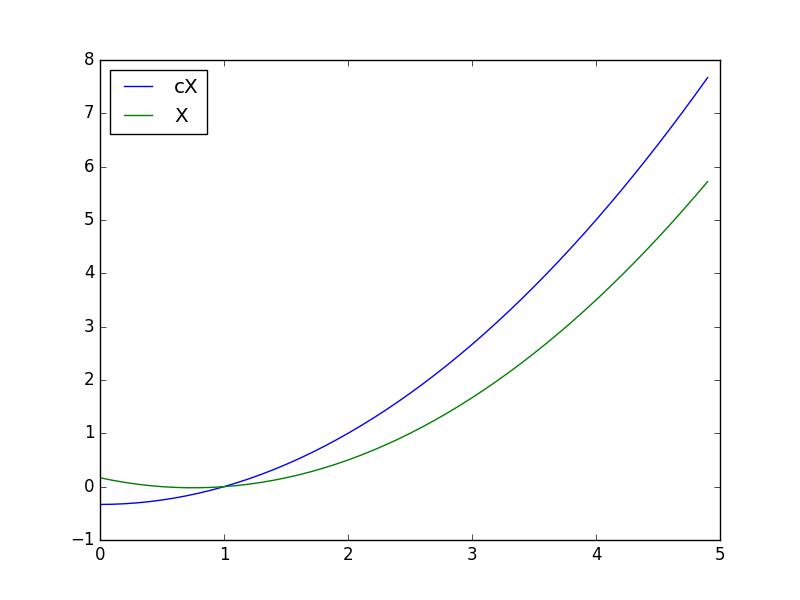
\includegraphics{q7}

\end{enumerate}

\subsection{Question 8, Rice 8.51}
The double exponential distribution is

\[ f(x\mid \theta) = \frac{1}{2} e^{-|x-\theta|} , \ -\infty < x < \infty \]

For an i.i.d. sample of size \marginnote{Is the point of $n=2m+1$ to imply that the sample is atleast 3?}$n=2m+1$, show that the mle of $\theta$ is the median of the sample.

Suppose we have a bunch of data $X_1, X_2,...,X_n$ which are iid variables with outcomes $x_1, x_2,...,x_n$.  Then
\begin{align*}
f(x_1, x_2,...,x_n \mid \theta) &= f(x_1\mid \theta)\cdot f(x_2\mid \theta)\cdot \cdot \cdot f(x_n \mid \theta)\\
&= \frac{1}{2}e^{-|x_1 - \theta|} \cdot \frac{1}{2}e^{-|x_2 - \theta|} \cdot \cdot \cdot \frac{1}{2}e^{-|x_n - \theta|}\\
&= \frac{1}{2^n} e^{-\sum_{i=1}^n|x_i -\theta|}
\end{align*}

Hence
\[ L(\theta) = \frac{1}{2^n} e^{-\sum_{i=1}^n|x_i -\theta|} \]

Which can be maximized by minimizing the exponent term

\[ g(\theta) = \sum_{n=1}^n |x_i-\theta|. \]

However, as warned this function is not differetiable as is.  A plot for small N reveals reveals that the slope changes at each instance where $x_i=\theta$.

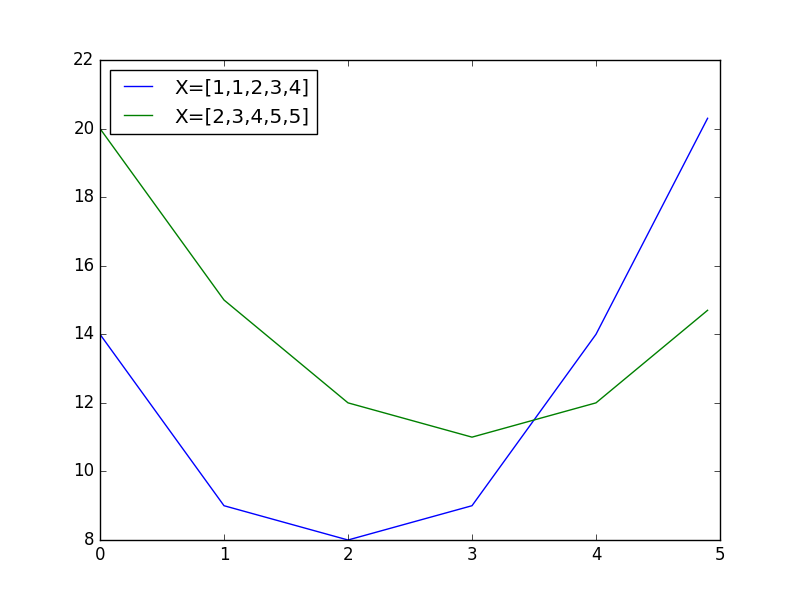
\includegraphics{q8.png}

It also appears that the function achieves a minimum when $\theta$ is equal to the median.

Let
\[ h(x, \theta) =
\begin{cases}
1 &\text { if }  x_i < \theta \\
-1 &\text { if } x_i > \theta \\
0 &\text {otherwise}\\
\end{cases}
\]

Then we have

\[ \frac{d g(\theta)}{d\theta} = \sum_{i=1}^n(h(x_i, \theta)) \]

Which will be positive if $\theta$ is greater than median of the data and negative if $\theta$ is less than the median of the data.  Which implies that the $L(\theta)$ function is maximized at the median, i.e. when $\hat{\theta} = \text{median}(x_i)$.
\end{document}
\grid
